 \begin{solution}

\begin{enumerate}
\item {[7 points]} Let
\[
\psi_0(x)=1
\]
and let
\[
\psi_n(x) = \sqrt{2} \cos\left(n\pi x\right)
\]
for $n=1,2,\ldots$. The spectral method yields the series solution
\[
\tilde{u}(x,t)=\sum_{n=0}^\infty a_n(t)\psi_n(x)
\]
where
\begin{eqnarray*}
a_0(t)&=&\int_0^10\,dx+\int_0^t\int_0^1f(x,s)\psi_0(x)\,dx\,ds
\\
&=&\int_0^t\int_0^1f(x,s)\psi_0(x)\,dx\,ds
\end{eqnarray*}
and
\begin{eqnarray*}
a_n(t)&=&\int_0^10\,dx e^{-n^2\pi^2t}+\int_0^te^{n^2\pi^2\left(s-t\right)}\int_0^1f(x,s)\psi_n(x)\,dx\,ds
\\
&=&\int_0^te^{n^2\pi^2\left(s-t\right)}\int_0^1f(x,s)\psi_n(x)\,dx\,ds
\end{eqnarray*}
for $n=1,2,\ldots$.

Now,
\begin{eqnarray*}
&&\int_0^1f(x,s)\psi_0(x)\,dx 
\\
&=& \left(\int_0^{1/2} f(x,s)\,dx+\int_{1/2}^1 f(x,s)\,dx\right)
\\
&=& 2\left(\int_0^{1/2} x\,dx+\int_{1/2}^1 1-x\,dx\right)
\\
&=& 2\left(\left[{1 \over 2}x^2\right]_0^{1/2}+\left[x-{1 \over 2}x^2\right]_{1/2}^1\right)
\\
&=& 2\left({1 \over 8}-0+1-{1 \over 2}-{1 \over 2}+{1 \over 8}\right)
\\
&=& 2\left({1 \over 8}+{8 \over 8}-{4 \over 8}-{4 \over 8}+{1 \over 8}\right)
\\
&=& {4 \over 8}
\\
&=& {1 \over 2}.
\end{eqnarray*}
Consequently,
\begin{eqnarray*}
a_0(t)&=&\int_0^t\int_0^1f(x,s)\psi_0(x)\,dx\,ds
\\
&=&\int_0^t{1 \over 2}\,ds
\\
&=&\left[{1 \over 2}s\right]_{s=0}^{s=t}
\\
&=&{1 \over 2}t.
\end{eqnarray*}

Also, for $n=1,2,3,\ldots$,
\begin{eqnarray*}
&&\int_0^1f(x,s)\psi_n(x)\,dx 
\\
&=& \sqrt{2}\left(\int_0^{1/2} f(x,s)\cos(n\pi x)\,dx+\int_{1/2}^1 f(x,s)\cos(n\pi x)\,dx\right)
\\
&=& 2\sqrt{2}\left(\int_0^{1/2} x\cos(n\pi x)\,dx+\int_{1/2}^1 (1-x)\cos(n\pi x)\,dx\right)
\\
&=&2\sqrt{2}\left(\left[{1 \over n\pi}x\sin(n\pi x)\right]_0^{1/2}-{1 \over n\pi}\int_0^{1/2} \sin(n\pi x)\,dx+\left[{1 \over n\pi}(1-x)\sin(n\pi x)\right]_{1/2}^1+{1 \over n\pi}\int_{1/2}^1 \sin(n\pi x)\,dx\right)
\\
&=&2\sqrt{2}\left({1 \over 2n\pi}\sin\left({n\pi \over 2} x\right)-{1 \over n\pi}\int_0^{1/2} \sin(n\pi x)\,dx-{1 \over 2n\pi}\sin\left({n\pi \over 2} x\right)+{1 \over n\pi}\int_{1/2}^1 \sin(n\pi x)\,dx\right)
\\
&=&{2\sqrt{2} \over n\pi}\left(\int_{1/2}^1 \sin(n\pi x)\,dx-\int_0^{1/2} \sin(n\pi x)\,dx\right)
\\
&=&{2\sqrt{2} \over n\pi}\left(\left[-{1 \over n\pi}\cos(n\pi x)\right]_{1/2}^1-\left[-{1 \over n\pi}\cos(n\pi x)\right]_0^{1/2}\right)
\\
&=&{2\sqrt{2} \over n\pi}\left(-{1 \over n\pi}\cos(n\pi)+{1 \over n\pi}\cos\left({n\pi \over 2}\right)+{1 \over n\pi}\cos\left({n\pi \over 2}\right)-{1 \over n\pi}\right)
\\
&=&{2\sqrt{2} \over n^2\pi^2}\left(2\cos\left({n\pi \over 2}\right)-\cos(n\pi)-1\right).
\end{eqnarray*}
Consequently,
\begin{eqnarray*}
a_n(t)&=&\int_0^te^{n^2\pi^2\left(s-t\right)}\int_0^1f(x,s)\psi_n(x)\,dx\,ds
\\
&=&{2\sqrt{2} \over n^2\pi^2}\left(2\cos\left({n\pi \over 2}\right)-\cos(n\pi)-1\right)\int_0^te^{n^2\pi^2\left(s-t\right)}\,ds
\\
&=&{2\sqrt{2} \over n^2\pi^2}\left(2\cos\left({n\pi \over 2}\right)-\cos(n\pi)-1\right)\left[\frac{1}{n^2\pi^2}e^{n^2\pi^2\left(s-t\right)}\right]_{s=0}^{s=t}
\\
&=&{2\sqrt{2} \over n^2\pi^2}\left(2\cos\left({n\pi \over 2}\right)-\cos(n\pi)-1\right)\left(\frac{1}{n^2\pi^2}-\frac{1}{n^2\pi^2}e^{-n^2\pi^2t}\right)
\\
&=&{2\sqrt{2} \over n^4\pi^4}\left(2\cos\left({n\pi \over 2}\right)-\cos(n\pi)-1\right)\left(1-e^{-n^2\pi^2t}\right)
\end{eqnarray*}
for $n=1,2,\ldots$.

Hence,
\[
\tilde{u}(x,t)={1 \over 2}t+\sum_{n=1}^\infty{4 \over n^4\pi^4}\left(2\cos\left({n\pi \over 2}\right)-\cos(n\pi)-1\right)\left(1-e^{-n^2\pi^2t}\right)\cos(n\pi x).
\]

\item {[5 points]} The requested plot is below.

\begin{center}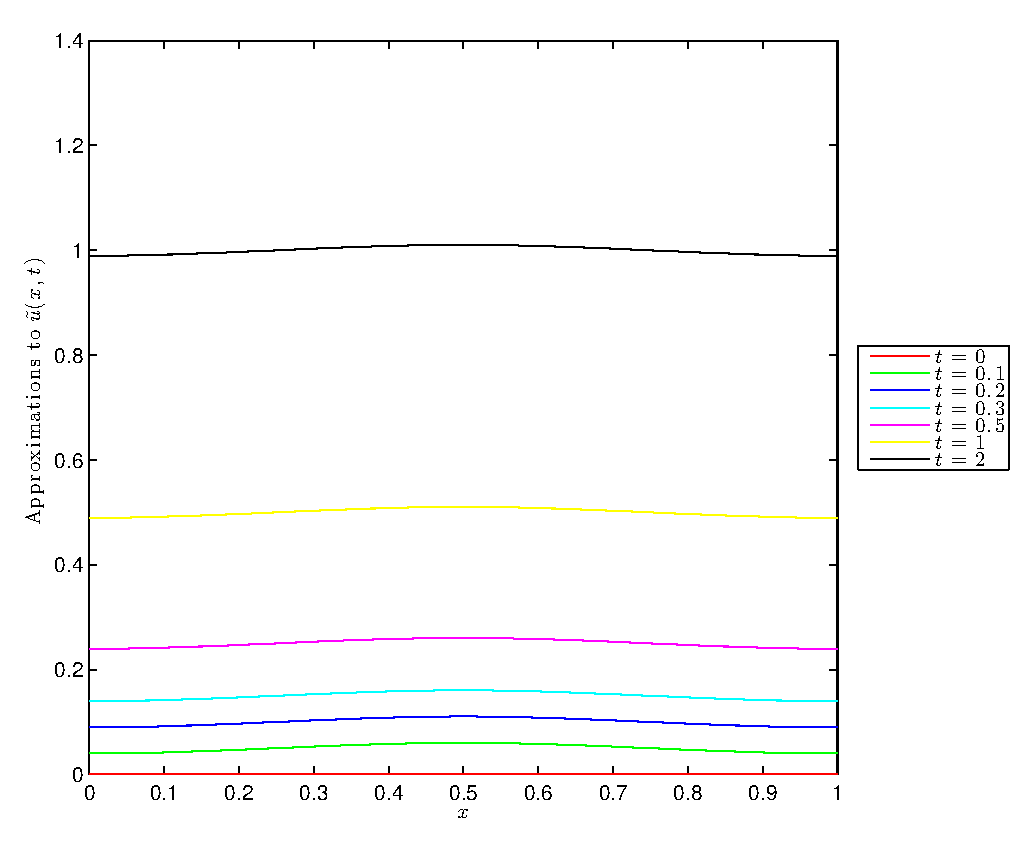
\includegraphics[scale=0.7]{hw39b.eps}\end{center}

The above plot was produced using the following MATLAB code.

\lstinputlisting{HW39b.m}

\item {[8 points]} Let
\[
w(x)=x^2
\]
so that
\[
w'(0)=0
\]
and
\[
w'(1)=2.
\]
Moreover, let $\hat{u}(x,t)$ be such that
\[
\hat{u}_t(x,t)-\hat{u}_{xx}(x,t) = f(x,t)+w''(x)=f(x,t)+2,\quad 0<x<1,\quad t>0;
\]
\[
\hat{u}(0,t) = \hat{u}(1,t) = 0,\quad t\ge0;
\]
and
\[
\hat{u}(x,0)=x^2-x^2=0,\quad 0<x<1.
\]
Then $u(x,t)=w(x)+\hat{u}(x,t)$ will be such that
\[
u_t(x,t)-u_{xx}(x,t)=\hat{u}_t(x,t)-w''(x)-\hat{u}_{xx}(x,t) = f(x,t)+2-2 = f(x,t),\quad 0<x<1,\quad t>0;
\]
\[
u_x(0,t) = w'(0) + \hat{u}_x(0,t) = 0+0 = 0,\quad t\ge0;
\]
\[
u_x(1,t) = w'(1) + \hat{u}_x(1,t) = 2+0 = 2,\quad t\ge0;
\]
and
\[
u(x,0)=w(x)+\hat{u}(x,0)=x^2+0=x^2,\quad 0<x<1.
\]
The spectral method yields that
\[
\hat{u}(x,t)=\sum_{n=0}^\infty \hat{a}_n(t)\psi_n(x)
\]
where
\begin{eqnarray*}
\hat{a}_0(t)&=&\int_0^10\,dx+\int_0^t\int_0^1\left(f(x,s)+2\right)\psi_0(x)\,dx\,ds
\\
&=&\int_0^t\int_0^1\left(f(x,s)+2\right)\psi_0(x)\,dx\,ds
\end{eqnarray*}
and
\begin{eqnarray*}
\hat{a}_n(t)&=&\int_0^10\,dx e^{-n^2\pi^2t}+\int_0^te^{n^2\pi^2\left(s-t\right)}\int_0^1\left(f(x,s)+2\right)\psi_n(x)\,dx\,ds
\\
&=&\int_0^te^{n^2\pi^2\left(s-t\right)}\int_0^1\left(f(x,s)+2\right)\psi_n(x)\,dx\,ds
\end{eqnarray*}
for $n=1,2,3,\ldots$.

Now,
\[
\int_0^1 2\psi_0(x)\,dx= 2\int_0^1\psi_0(x)\psi_0(x)\,dx=2
\]
and in part (a) we computed that
\[
\int_0^t\int_0^1f(x,s)\psi_0(x)\,dx\,ds={1 \over 2}t
\]
and so, for $n=1,2,3,\ldots$,
\[
\int_0^t\int_0^1\left(f(x,s)+2\right)\psi_0(x)\,dx\,ds={1 \over 2}t+\int_0^t2\,ds={1 \over 2}t+\left[2s\right]_{s=0}^{s=t}={1 \over 2}t+2t={1 \over 2}t+{4 \over 2}t={5 \over 2}t.
\]
Consequently,
\begin{eqnarray*}
\hat{a}_0(t)&=&\int_0^t\int_0^1\left(f(x,s)+2\right)\psi_0(x)\,dx\,ds
\\
&=&{5 \over 2}t.
\end{eqnarray*}

Also, for $n=1,2,3,\ldots$,
\[
\int_0^1 2\psi_n(x)\,dx= 2\int_0^1\psi_0(x)\psi_n(x)\,dx=0
\]
and in part (a) we computed that, for $n=1,2,3,\ldots$,
\[
\int_0^te^{n^2\pi^2\left(s-t\right)}\int_0^1f(x,s)\psi_n(x)\,dx\,ds=\frac{4\sqrt{2}}{n^4\pi^4}\sin\left(\frac{n\pi}{2}\right)\left(1-e^{-n^2\pi^2t}\right)
\]
and so, for $n=1,2,3,\ldots$,
\[
\int_0^te^{n^2\pi^2\left(s-t\right)}\int_0^1\left(f(x,s)+2\right)\psi_n(x)\,dx\,ds=\frac{4\sqrt{2}}{n^4\pi^4}\sin\left(\frac{n\pi}{2}\right)\left(1-e^{-n^2\pi^2t}\right).
\]
Consequently,
\begin{eqnarray*}
\hat{a}_n(t)&=&\int_0^te^{n^2\pi^2\left(s-t\right)}\int_0^1\left(f(x,s)+2\right)\psi_n(x)\,dx\,ds
\\
&=&{2\sqrt{2} \over n^4\pi^4}\left(2\cos\left({n\pi \over 2}\right)-\cos(n\pi)-1\right)\left(1-e^{-n^2\pi^2t}\right)
\end{eqnarray*}
for $n=1,2,3,\ldots$.


Hence,
\[
u(x,t)=x^2+{5 \over 2}t+\sum_{n=1}^\infty {4 \over n^4\pi^4}\left(2\cos\left({n\pi \over 2}\right)-\cos(n\pi)-1\right)\left(1-e^{-n^2\pi^2t}\right)\cos(n\pi x).
\]

\item {[5 points]} The requested plot is below.

\begin{center}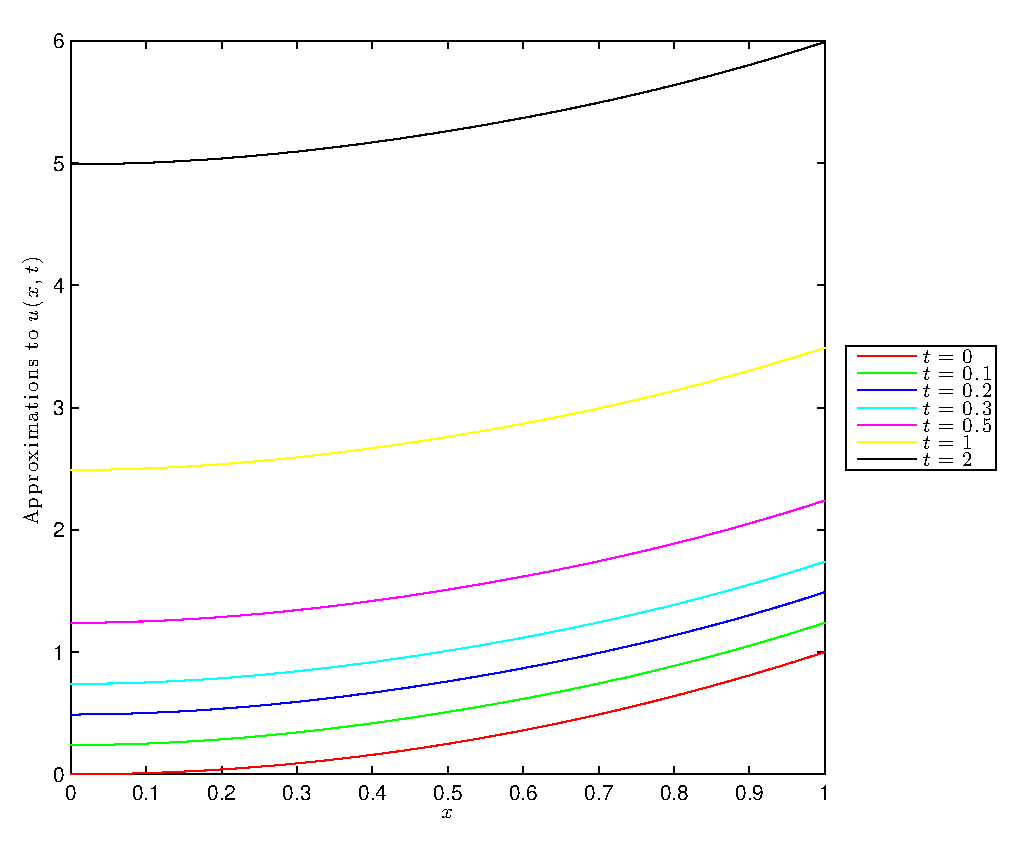
\includegraphics[scale=0.7]{hw39d.eps}\end{center}

The above plot was produced using the following MATLAB code.

\lstinputlisting{HW39d.m}

\end{enumerate}

\end{solution}